\documentclass{scrartcl}
\usepackage[utf8]{inputenc}
\usepackage[T1]{fontenc}      
\usepackage[francais]{babel}
% Layout and figures
\usepackage[top=2.5cm,bottom=2.5cm,right=2.5cm,left=2.5cm]{geometry}
\usepackage{subfigure}
\usepackage{rotating}
% Math
\usepackage{amsmath}
\usepackage{amssymb}
\usepackage{amsthm}
% Links
\usepackage{url}
\usepackage{hyperref}
\hypersetup{
    colorlinks,
    citecolor=black,
    filecolor=black,
    linkcolor=black,
    urlcolor=black
}
% New commands
\newcommand{\annexe}{\part{Annexes}\appendix}
\newcommand{\biblio}[1]{\bibliographystyle{plain}\bibliography{#1}\nocite{*}}

\newcommand{\doctitle}[1]{
	\title{LSINF1225 - Projet BarTender}
	\subtitle{#1}
	\author{\textbf{Groupe T}\\
	\textsc{Gérard} Louis (6317-12-00)\\
	\textsc{Gillon} Bastien (5937-12-00)\\
	\textsc{Jacques} Thibault (2954-13-00)\\
	\textsc{Paris} Antoine (3158-13-00)\\
	\textsc{Ramelot} Sylvain (4763-13-00)}
	\date{\today}

	\begin{document}

	\maketitle
	%\tableofcontents
}

% For the same reason as in UML-diagram.tex
% no title here
%\doctitle{Diagramme UML de séquence}
\begin{document}

\begin{figure}
	\centering
	\rotatebox{90}{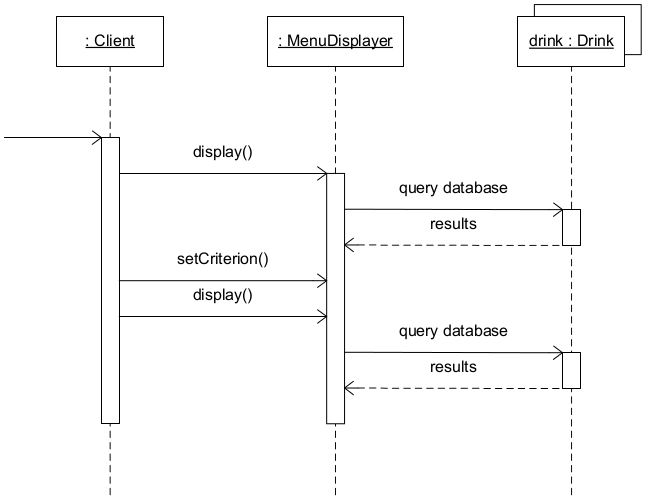
\includegraphics[scale=0.6]{UML-sequence/UML-sequence-1.png}}
\end{figure}

\begin{figure}
	\centering
	\rotatebox{90}{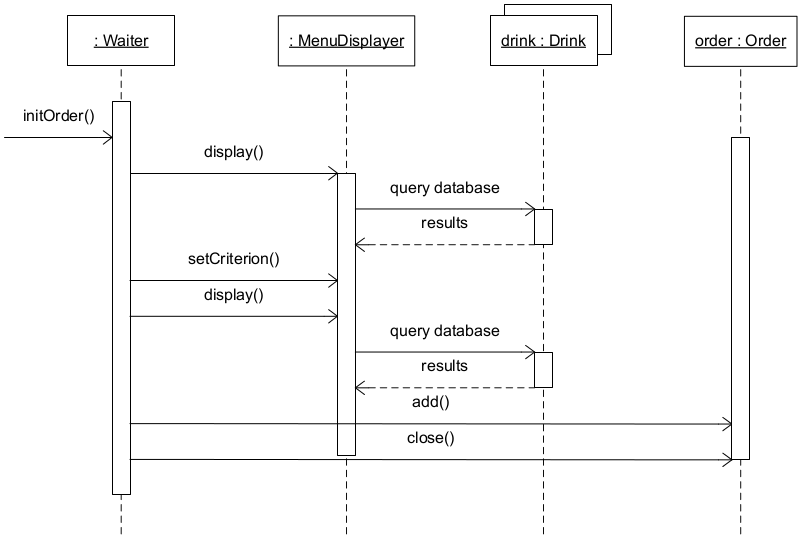
\includegraphics[scale=0.6]{UML-sequence/UML-sequence-2.png}}
\end{figure}

\begin{figure}
	\centering
	\rotatebox{90}{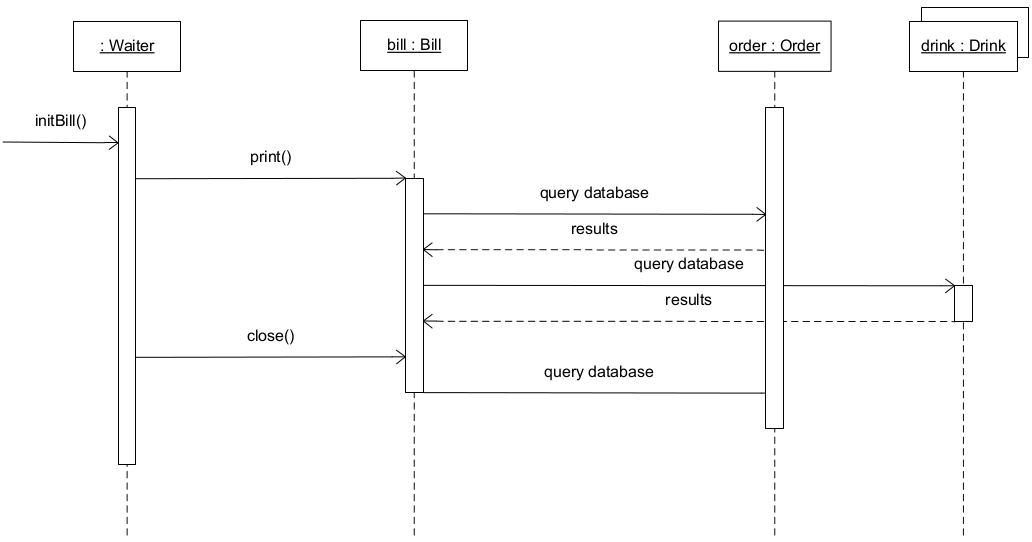
\includegraphics[scale=0.6]{UML-sequence/UML-sequence-3.png}}
\end{figure}

\begin{figure}
	\centering
	\rotatebox{90}{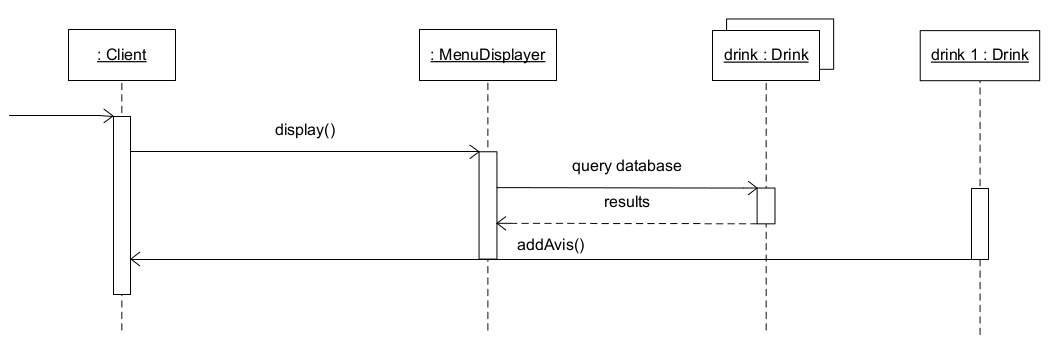
\includegraphics[scale=0.6]{UML-sequence/UML-sequence-4.png}}
\end{figure}

\input{../footer.tex}